\documentclass[tikz,border=3mm]{standalone}
\usetikzlibrary{arrows.meta,calc,positioning}
\begin{document}
\pagecolor{white}
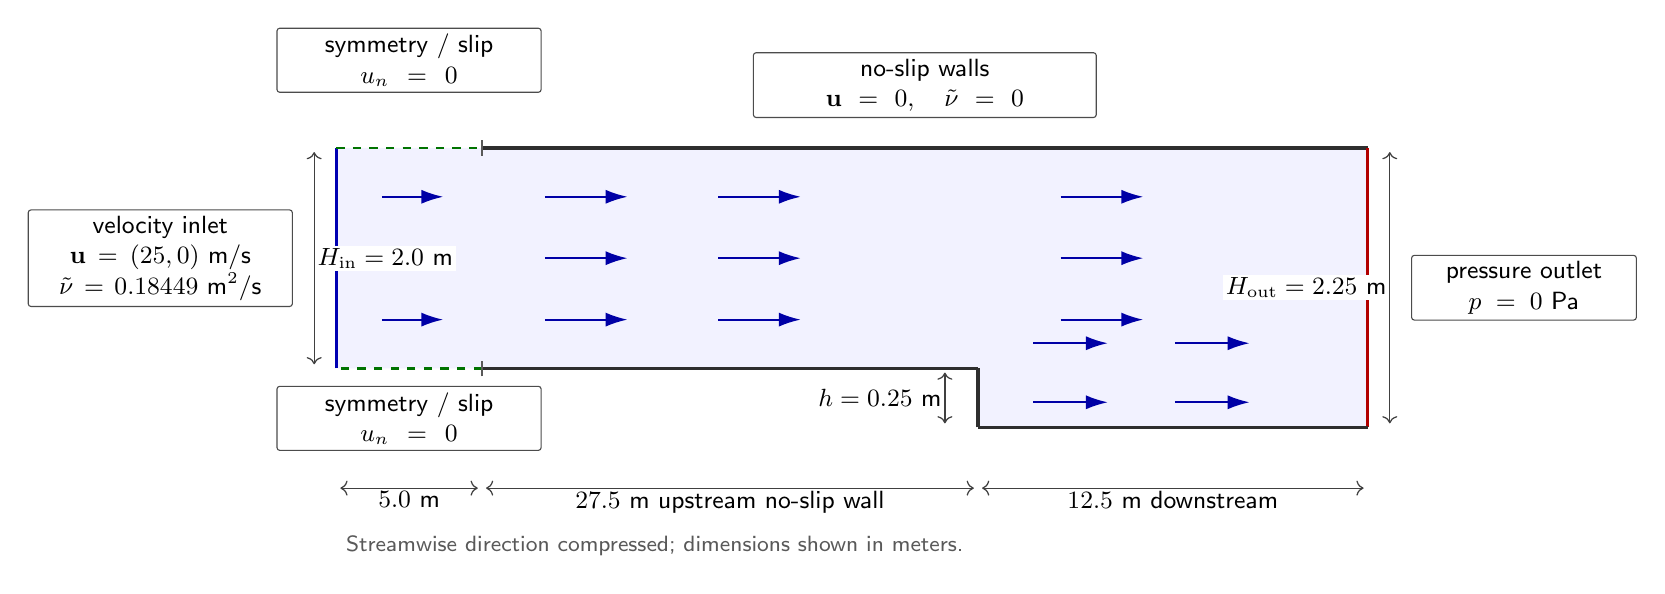
\begin{tikzpicture}[
  font=\sffamily\small,
  flow/.style={-{Latex[length=2.8mm,width=1.8mm]}, line width=0.72pt, draw=blue!65!black},
  dim/.style={<->, line width=0.45pt, draw=black!75, shorten <=1.5pt, shorten >=1.5pt},
  wall/.style={line width=1.25pt, draw=black!82},
  sym/.style={line width=1.0pt, draw=green!45!black, dashed},
  inlet/.style={line width=1.1pt, draw=blue!70!black},
  outlet/.style={line width=1.1pt, draw=red!70!black},
  bc/.style={draw=black!70, fill=white, rounded corners=1pt, inner sep=2.2pt, align=center}
]

% Streamwise lengths are compressed for readability.
\def\xin{0.0}
\def\xwall{1.85}
\def\xstep{8.15}
\def\xout{13.10}
\def\yb{-0.75}
\def\y0{0.0}
\def\yt{2.80}

% Fluid domain.
\fill[blue!5] (\xin,\y0) -- (\xin,\yt) -- (\xout,\yt) -- (\xout,\yb)
  -- (\xstep,\yb) -- (\xstep,\y0) -- cycle;

% Boundary-condition segments.
\draw[inlet] (\xin,\y0) -- (\xin,\yt);
\draw[sym] (\xin,\yt) -- (\xwall,\yt);
\draw[wall] (\xwall,\yt) -- (\xout,\yt);
\draw[outlet] (\xout,\yb) -- (\xout,\yt);
\draw[wall] (\xout,\yb) -- (\xstep,\yb);
\draw[wall] (\xstep,\yb) -- (\xstep,\y0);
\draw[wall] (\xstep,\y0) -- (\xwall,\y0);
\draw[sym] (\xwall,\y0) -- (\xin,\y0);

% Split markers where symmetry changes to wall.
\draw[black!65, line width=0.45pt] (\xwall,\y0-0.10) -- (\xwall,\y0+0.10);
\draw[black!65, line width=0.45pt] (\xwall,\yt-0.10) -- (\xwall,\yt+0.10);

% Flow arrows, placed away from no-slip boundaries.
\foreach \y in {0.62,1.40,2.18} {
  \draw[flow] (0.58,\y) -- ++(0.78,0);
  \draw[flow] (2.65,\y) -- ++(1.05,0);
  \draw[flow] (4.85,\y) -- ++(1.05,0);
  \draw[flow] (9.20,\y) -- ++(1.05,0);
}
\foreach \y in {-0.43,0.32} {
  \draw[flow] (8.85,\y) -- ++(0.95,0);
  \draw[flow] (10.65,\y) -- ++(0.95,0);
}

% Boundary labels.
\node[bc, anchor=east, text width=32mm] at (\xin-0.55,{0.5*\yt})
  {velocity inlet\\$\mathbf{u}=(25,0)$ m/s\\$\tilde{\nu}=0.18449$ m$^2$/s};
\node[bc, anchor=west, text width=27mm] at (\xout+0.55,{0.5*(\yb+\yt)})
  {pressure outlet\\$p=0$ Pa};
\node[bc, anchor=south, text width=32mm] at ({0.5*(\xin+\xwall)},{\yt+0.70})
  {symmetry / slip\\$u_n=0$};
\node[bc, anchor=north, text width=32mm] at ({0.5*(\xin+\xwall)},{\y0-0.22})
  {symmetry / slip\\$u_n=0$};
\node[bc, anchor=south, text width=42mm] at ({0.5*(\xwall+\xout)},{\yt+0.38})
  {no-slip walls\\$\mathbf{u}=0,\quad \tilde{\nu}=0$};

% Dimensions.
\draw[dim] (\xin,-1.52) -- node[below, fill=white, inner sep=1pt]
  {$5.0$ m} (\xwall,-1.52);
\draw[dim] (\xwall,-1.52) -- node[below, fill=white, inner sep=1pt]
  {$27.5$ m upstream no-slip wall} (\xstep,-1.52);
\draw[dim] (\xstep,-1.52) -- node[below, fill=white, inner sep=1pt]
  {$12.5$ m downstream} (\xout,-1.52);

\draw[dim] (\xin-0.28,\y0) -- node[right, fill=white, inner sep=1pt]
  {$H_\mathrm{in}=2.0$ m} (\xin-0.28,\yt);
\draw[dim] (\xout+0.28,\yb) -- node[left, fill=white, inner sep=1pt]
  {$H_\mathrm{out}=2.25$ m} (\xout+0.28,\yt);
\draw[dim] (\xstep-0.42,\yb) -- node[left, fill=white, inner sep=1pt]
  {$h=0.25$ m} (\xstep-0.42,\y0);

\node[anchor=west, text=black!65, font=\sffamily\footnotesize] at (\xin,-2.26)
  {Streamwise direction compressed; dimensions shown in meters.};

\end{tikzpicture}
\end{document}
